\begin{figure}[!h]
  \vskip -0.25cm
  \begin{center}
    \ifshort
    %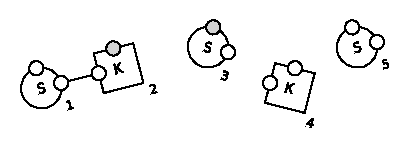
\includegraphics[scale=1.0]{figures/mixture-compact.pdf}
    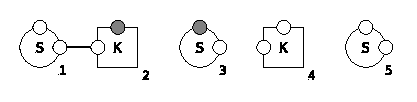
\includegraphics[scale=1.0]{figures/mixture-linear.pdf}
    \else
    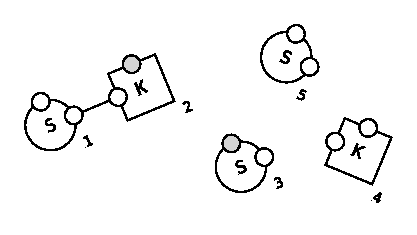
\includegraphics[scale=0.9]{figures/mixture.pdf}
    \fi
  \end{center}
  \vskip -0.5cm
\caption{A mixture graph. Sites are here identified by their position on
agents instead of a name. 
% removed "longversion", since it only repeated what the previous sentence asserts.} 
A grey site indicates a phosphorylated state. Numbers
are global agent identifiers in the mixture.}
  \label{fig:mixture}
\end{figure}